\documentclass[10pt,a4paper]{article}
\usepackage[a4paper,margin=2.2cm]{geometry}
\usepackage[T1]{fontenc}
\usepackage{lmodern}
\usepackage{amsmath,amssymb,bm}
\usepackage{graphicx}
\usepackage{booktabs}
\usepackage{tabularx}
\usepackage{enumitem}
\usepackage{xcolor}
\usepackage{caption}
\usepackage{float}
\usepackage{tikz}
\usetikzlibrary{positioning,arrows.meta,shapes.geometric,fit,calc}
\usepackage[colorlinks=true,linkcolor=blue!50!black,urlcolor=blue!50!black,citecolor=blue!50!black]{hyperref}

\setlist{itemsep=2pt,topsep=3pt}
\newcommand{\meas}{\textsc{measured}}
\newcommand{\inh}{\textsc{inherited}}
\newcommand{\est}{\textsc{estimated}}
\newcommand{\hyp}{\textsc{hypothesis}}
\newcommand{\x}{\bm{x}}
\newcommand{\Pm}{\mathbf{P}}
\newcommand{\Fm}{\mathbf{F}}
\newcommand{\Qm}{\mathbf{Q}}
\newcommand{\Hm}{\mathbf{H}}
\newcommand{\R}{\mathbb{R}}
\newcolumntype{L}{>{\raggedright\arraybackslash}X}

\title{\textbf{Ground-Truth Ego-Trajectory Reconstruction from Smartphone Dashcams}\\[4pt]
\large Architecture, estimation theory, findings, comparison with NVIDIA ViPE,\\ and a plan toward a fused geometric video engine}
\author{TrajectoryReconstruction / TanitAD --- technical report}
\date{8 November 2026}

\begin{document}
\maketitle

\begin{abstract}
\noindent We describe a pipeline that turns a consumer smartphone recording --- camera video plus IMU,
GNSS and orientation logs from the Sensor Logger app --- into ground-truth ego trajectories for training
end-to-end driving models, with a camera calibration that projects the trajectory into every frame.
The report gives the full estimation theory: how video and sensors are put on one clock (container
anchors refined by a three-band, three-axis gyro--image cross-correlation), how the phone's attitude in
the vehicle is recovered (gravity, centripetal acceleration and GNSS sign checks), and how motion data are
integrated into a trajectory: a six-state extended Kalman filter run forward over the whole session with
the gyro and accelerometer as inputs and GNSS position, speed and course as measurements, followed by a
Rauch--Tung--Striebel backward pass that gives every instant the information of the entire drive. We
derive the process and measurement models, the robust update, the standstill constraints, the rigid
transform from the phone's path to the rear axle, the steering read-out and the hold-out validation.
We then report what we measured on five recordings from three phones, including a recording from a
Galaxy S24 Ultra in an Audi A6 e-tron made with the ultra-wide lens, compare the approach with NVIDIA's
ViPE (arXiv:2508.10934), and set out a plan that adopts ViPE's methods inside an estimator that keeps
inertial and GNSS metric scale, explicit time synchronisation and a vehicle and road model.
Numbers carry their evidence class: \meas{} (ours, with the artifact), \inh{} (another source, not
re-verified), \est{}, or \hyp.
\end{abstract}

\tableofcontents
\clearpage

%=====================================================================
\section{Problem and output}

For every video frame the pipeline outputs the vehicle's past and future trajectory in an ego frame over
$t \in [-3, +5]$\,s: positions, heading, speed and positional uncertainty, together with the steering-wheel
angle implied by the motion, a bird's-eye view and the future path drawn into the image. The ego frame is
FLU (ISO\,8855: $x$ forward, $y$ left, $z$ up) with its origin at the rear axle at the reference instant.

The inputs are deliberately cheap: a phone in a windscreen holder recording with Sensor Logger. There is no
vehicle CAN, no calibration target and no control over the camera mode the app uses. Two consequences
drive the design: the pipeline must \emph{refuse} recordings that cannot yield trustworthy ground truth,
and it must recover all geometry --- time offset, mount attitude, intrinsics --- from the drive itself.

%=====================================================================
\section{Architecture}
\label{sec:arch}

\begin{figure}[H]
\centering
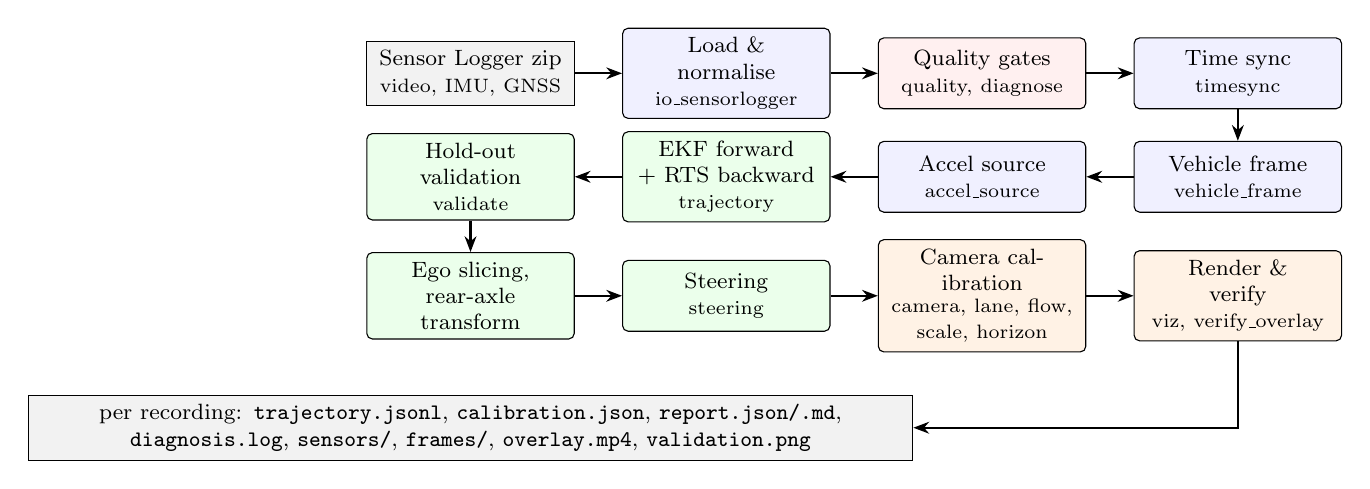
\begin{tikzpicture}[
  node distance=4mm and 6mm,
  box/.style={draw, rounded corners=2pt, align=center, font=\footnotesize, minimum height=9mm, text width=24mm, fill=#1},
  box/.default=white,
  io/.style={draw, align=center, font=\footnotesize, minimum height=8mm, text width=24mm, fill=gray!10},
  arr/.style={-{Stealth[length=2mm]}, thick}]
\node[io] (zip) {Sensor Logger zip\\ \scriptsize video, IMU, GNSS};
\node[box=blue!6, right=of zip] (load) {Load \&\\ normalise\\ \scriptsize io\_sensorlogger};
\node[box=red!6, right=of load] (qc) {Quality gates\\ \scriptsize quality, diagnose};
\node[box=blue!6, right=of qc] (sync) {Time sync\\ \scriptsize timesync};
\node[box=blue!6, below=of sync] (vf) {Vehicle frame\\ \scriptsize vehicle\_frame};
\node[box=blue!6, left=of vf] (acc) {Accel source\\ \scriptsize accel\_source};
\node[box=green!8, left=of acc] (ekf) {EKF forward\\ + RTS backward\\ \scriptsize trajectory};
\node[box=green!8, left=of ekf] (val) {Hold-out\\ validation\\ \scriptsize validate};
\node[box=green!8, below=of val] (ego) {Ego slicing,\\ rear-axle transform};
\node[box=green!8, right=of ego] (steer) {Steering\\ \scriptsize steering};
\node[box=orange!10, right=of steer] (cam) {Camera calibration\\ \scriptsize camera, lane, flow,\\ \scriptsize scale, horizon};
\node[box=orange!10, right=of cam] (rend) {Render \&\\ verify\\ \scriptsize viz, verify\_overlay};
\node[io, below=7mm of ego, text width=110mm] (out) {per recording: \texttt{trajectory.jsonl}, \texttt{calibration.json},
  \texttt{report.json/.md}, \texttt{diagnosis.log}, \texttt{sensors/}, \texttt{frames/}, \texttt{overlay.mp4}, \texttt{validation.png}};
\draw[arr] (zip) -- (load); \draw[arr] (load) -- (qc); \draw[arr] (qc) -- (sync);
\draw[arr] (sync) -- (vf); \draw[arr] (vf) -- (acc); \draw[arr] (acc) -- (ekf); \draw[arr] (ekf) -- (val);
\draw[arr] (val) -- (ego); \draw[arr] (ego) -- (steer); \draw[arr] (steer) -- (cam); \draw[arr] (cam) -- (rend);
\draw[arr] (rend.south) |- (out.east);
\end{tikzpicture}
\caption{Data flow. Blue: data preparation; red: refusal gates; green: trajectory; orange: camera and
rendering. The sync result feeds both the trajectory window and every frame's time stamp.}
\end{figure}

\paragraph{Driver.} \texttt{pipeline.py} consumes a folder of Sensor Logger \texttt{.zip} archives directly.
A registry keyed on each archive's input fingerprint makes runs resumable and idempotent: completed work
is skipped, failures are retried, changed inputs are reprocessed, and an interruption costs at most one
recording. Work happens in a local scratch directory and is published at the end (the source folder is a
Google Drive mount that has dropped out mid-run). Each recording is \emph{diagnosed before any solving};
a rejected recording keeps its written analysis.

\begin{table}[H]
\centering\small
\begin{tabularx}{\textwidth}{@{}>{\raggedright\arraybackslash}p{4.6cm}L@{}}
\toprule
module & role \\
\midrule
\texttt{io\_sensorlogger} & loads all streams onto one timebase; detects platform, accelerometer units, iOS $-1$ sentinels \\
\texttt{quality}, \texttt{diagnose} & frozen GNSS, rates, gaps, motion, accelerometer usability; \textsc{ok}/\textsc{degraded}/\textsc{reject} with evidence \\
\texttt{timesync} & container PTS, coarse anchors, image angular rate, three-band gyro cross-correlation \\
\texttt{vehicle\_frame} & one phone$\to$vehicle rotation per session \\
\texttt{accel\_source} & tiered choice of longitudinal acceleration, with automatic quality scoring \\
\texttt{trajectory} & session EKF + RTS smoother; ego slicing; rigid transform to the rear axle \\
\texttt{validate} & $k$-fold GNSS hold-out and internal consistency \\
\texttt{steering} & curvature, bicycle model with understeer, rate limits, uncertainty \\
\texttt{camera}, \texttt{lane\_calib}, \texttt{scale\_calib}, \texttt{flow\_calib}, \texttt{horizon\_calib}, \texttt{plane\_calib}, \texttt{vp\_calib}, \texttt{ground\_calib} & intrinsics and mount from the video (\S\ref{sec:calib}) \\
\texttt{attitude\_track} & per-frame yaw/horizon for recordings with electronic stabilisation \\
\texttt{viz}, \texttt{tools/verify\_overlay} & ribbon and bird's-eye rendering; lane-based verification \\
\bottomrule
\end{tabularx}
\caption{Modules of the \texttt{trajlib} library.}
\end{table}

%=====================================================================
\section{Data model}

All streams are expressed in session time $t$ (\texttt{seconds\_elapsed}), seconds since the recording
epoch $T_0$ written in \texttt{Metadata.csv}; absolute time is $T_0 + t$. Platform conventions are detected
from the data: Android's gravity vector points up and iOS's down; iOS exports the raw accelerometer in $g$
(recognised by a mean norm of 1\,g), Android in m/s$^2$; iOS writes $-1$ for unavailable speed, course and
accuracy, which would otherwise poison the filter (one such value made a whole iOS state NaN).
GNSS fixes are converted to a local ENU tangent plane at the first fix (WGS-84 $\to$ ECEF $\to$ ENU).
Headings use the mathematical convention $\psi$ (counter-clockwise from East); a GNSS bearing $\beta$
(clockwise from North) maps to $\psi = \pi/2 - \beta$.

%=====================================================================
\section{Quality gates}
Before any solving: GNSS frozen fraction (byte-identical consecutive fixes --- one recording's 78 fixes were
all one cached fix), fix count and gaps, receiver accuracy, IMU rates, motion (distance travelled, moving
fraction), overlap of video and sensor data, and the usable accelerometer tier. A \textsc{reject} stops the
recording with its report; \textsc{degraded} proceeds with the reason recorded. The design rule is that a
silently wrong trajectory is worse than none, because it poisons a training set unnoticed.

%=====================================================================
\section{Time synchronisation}
\label{sec:sync}

Every frame needs a session time $t_k = t_0 + p_k$, where $p_k$ is the frame's presentation timestamp
(PTS) read from the container and $t_0$ the session time of the first frame. Using PTS rather than
$k/\text{fps}$ matters: at a measured 29.9436\,fps against a nominal 30, index arithmetic drifts 1.7\,s over
78\,s.

\paragraph{Coarse anchors.} Three candidates for $t_0$ are formed: the epoch encoded in the video file
name (\emph{container}), and the MP4 \texttt{creation\_time} $T_c$ read either as the start
($T_c - T_0$) or as the end ($T_c - T_0 - D$, with duration $D$). Android writes $T_c$ when the muxer
finalises the file (the end), iOS at the start; the first candidate inside a physically possible window
($-3$ to $+15$\,s) is used.

\paragraph{Image angular rate.} Corners are tracked with pyramidal Lucas--Kanade between consecutive frames
in a band that excludes sky and the static bonnet/dashboard (RANSAC would otherwise lock onto the static
majority). A partial-affine (similarity) transform is fitted; with a nominal focal length $f$, the camera's
incremental rotations are $\Delta\theta_\text{yaw} \approx t_x/f$, $\Delta\theta_\text{pitch} \approx t_y/f$
and $\Delta\theta_\text{roll}$ = the in-plane angle, giving $\bm\omega_\text{cam}(t) \in \R^3$. Forward
translation leaks into $t_x$, so the amplitude is unreliable; only the timing is used.

\paragraph{Three-axis lag and axis map.} Both signals are resampled on a common grid ($\Delta = 20$\,ms) and
band-passed with a zero-phase Butterworth filter (removes bias drift and high-frequency noise). For each
candidate lag $\tau \in [-3, 3]$\,s the gyro triad $\mathbf{B}(\tau) \in \R^{n\times3}$, sampled at
$t+\tau$, is mapped onto the camera triad $\mathbf{A} \in \R^{n\times3}$ by a free $3\times3$ matrix:
\begin{equation}
\mathbf{M}(\tau) = \arg\min_{\mathbf{M}} \|\mathbf{A} - \mathbf{B}(\tau)\mathbf{M}\|_F^2, \qquad
s(\tau) = 1 - \frac{\|\mathbf{A} - \mathbf{B}(\tau)\mathbf{M}(\tau)\|_F^2}{\|\mathbf{A}\|_F^2}.
\end{equation}
$\mathbf{M}$ is a general matrix rather than a rotation on purpose: it absorbs the unknown phone$\to$camera
axis mapping \emph{and} the per-axis gain error of the image rates. The score $s$ is the fraction of
camera-signal variance explained; $\hat\tau = \arg\max s$, refined to sub-sample precision by a parabola
through the peak: $\hat\tau \mathrel{+}= \Delta\,\tfrac12 (s_{-} - s_{+})/(s_{-} - 2s_0 + s_{+})$.

\paragraph{Acceptance.} The fit is repeated in three bands, $[0.02,1]$, $[0.05,2]$ and $[0.10,3]$\,Hz. A true
lag is band-independent; a spurious peak moves. The refinement is accepted only if the three lags agree
within 100\,ms and the peak score exceeds 0.10; then $t_0 \leftarrow t_0 + \operatorname{median}(\hat\tau)$,
otherwise the coarse anchor is kept and the rejection is recorded.

\begin{table}[H]
\centering\small
\begin{tabular}{@{}lccl@{}}
\toprule
recording & old pipeline (first GNSS fix) & this method & agreement \\
\midrule
2025-08-14 & 0.606\,s & 0.2134\,s & 3 bands within 1\,ms, score 0.59 \\
2025-08-11 & 1.037\,s & 0.7327\,s & 3 bands within 96\,ms, score 0.89 \\
Pacific Coast Hwy (iPhone 14) & --- & 0.1068\,s & within 7\,ms, score 0.93 \\
2026-11-03 1000N (S24 Ultra) & --- & 0.47\,s & within 35\,ms, score 0.82 (\meas) \\
\bottomrule
\end{tabular}
\caption{Video start in session time (first three rows \inh{} from AUDIT.md).}
\end{table}

%=====================================================================
\section{Phone-to-vehicle frame}
\label{sec:vframe}

The phone sits at an unknown attitude, fixed for the session. One rotation $\mathbf{R}_{vp}$ (phone to
vehicle) is estimated from all the data, with its three axes found independently:
\begin{itemize}
\item \textbf{Up} $\hat{\bm u}$: the mean of the gravity stream, $\hat{\bm u} = \overline{\bm g}/\|\overline{\bm g}\|$.
  Its sign is \emph{measured}: the rotation rate about $\hat{\bm u}$, $\omega_u = \bm\omega\cdot\hat{\bm u}$, is
  correlated with the GNSS heading rate $\dot\psi_\text{GNSS}$ over moving fixes; a negative correlation flips
  $\hat{\bm u}$. (Assuming Android's convention inverted every turn on iOS: $r=-0.43$ on Rose Ave.)
  Without a gravity stream, $\hat{\bm u}$ is the principal axis of the gyro signal, since a road vehicle
  rotates almost only in yaw.
\item \textbf{Left} $\hat{\bm l}$: from the centripetal relation $a_\text{lat} = v\,\omega_\text{up}$. With the
  horizontal linear acceleration $\bm a_h = \bm a - (\bm a\cdot\hat{\bm u})\hat{\bm u}$ and a speed gate $w(t)$,
  \begin{equation}
  \hat{\bm l} \propto \Big(\textstyle\sum_t w_t\,\omega_{\text{up},t}\,\bm a_{h,t}\Big)_{\perp \hat{\bm u}},
  \end{equation}
  the horizontal direction whose acceleration best correlates with the yaw rate. The normalised
  correlation is reported as \texttt{lateral\_score}.
\item \textbf{Forward} $\hat{\bm f} = \hat{\bm l} \times \hat{\bm u}$ (right-handed FLU). Its sign is fixed by the
  camera boresight (the rear camera looks along $-z_\text{phone}$, which has a positive forward component),
  and checked against the GNSS longitudinal acceleration when GNSS is healthy.
\end{itemize}
Then $\mathbf{R}_{vp} = [\hat{\bm f}\;\hat{\bm l}\;\hat{\bm u}]^\top$ and any phone-frame vector maps as
$\bm v_\text{veh} = \mathbf{R}_{vp}\bm v_\text{phone}$. The vehicle yaw rate used by the filter is
$\omega = (\mathbf{R}_{vp}\bm\omega_\text{gyro})_z$.

%=====================================================================
\section{Longitudinal acceleration}
\label{sec:accel}

Android's \texttt{Accelerometer} stream is \emph{linear} acceleration: specific force minus a continuously
re-estimated gravity whose time constant is about a second, so sustained acceleration leaks into the
gravity estimate and is subtracted away. Measured on 2025-08-11 its forward component integrates to
$-0.8$\,m/s while the car gained $+7.8$\,m/s (correlation with GNSS $dv/dt$: $-0.06$). The source is
therefore chosen in tiers:
\begin{enumerate}
\item raw specific force $\bm a^\text{tot}$ with gravity removed through the gyro-led attitude quaternion,
  $\bm a = \mathbf{R}(q)^{\!\top}\bm a^\text{tot} - \bm g$ in the world frame;
\item $\bm a^\text{tot}$ minus the \texttt{Gravity} stream;
\item the linear stream;
\item none: $a_f \equiv 0$ and the process noise is raised so speed is a random walk driven by GNSS.
\end{enumerate}
Each candidate's forward component $a_f = (\mathbf{R}_{vp}\bm a)_x$ is scored by its agreement with
GNSS-derived acceleration; a source below the quality threshold is disabled rather than allowed to inject
noise. Unknown quality (e.g.\ NaN from a single missing speed) is treated as unusable, not as trusted.

%=====================================================================
\section{Trajectory estimation: forward filtering and backward smoothing}
\label{sec:ekf}

\subsection{Why one session-level estimate}
The earlier implementation solved a fresh filter inside each frame's window $[t_k, t_k+5\,\text{s}]$: no
past, neighbouring frames 33\,ms apart disagreeing, $\approx$5 GNSS fixes per solve and 2\,GB of duplicated
sensor data per 78\,s. We instead estimate the \emph{whole session once} --- a forward pass that is causal,
then a backward pass that propagates future information --- and slice every frame's window from that single
smoothed solution. Every frame then carries the full past and future, and adjacent frames are consistent
by construction.

\subsection{State and motion model}
On a uniform grid with $\Delta t = 10$\,ms the state is
\begin{equation}
\x = [\,E,\; N,\; v,\; \psi,\; b_\omega,\; b_a\,]^\top \in \R^6,
\end{equation}
position in the ENU plane, forward speed, heading, gyro yaw-rate bias and longitudinal accelerometer bias.
The vehicle is non-holonomic (it moves along its heading). The control inputs are the vehicle-frame yaw
rate $\omega_k$ and longitudinal acceleration $a_{f,k}$. With $a = a_f - b_a$, $\tilde\omega = \omega - b_\omega$,
$c=\cos\psi$, $s=\sin\psi$, the discrete propagation is
\begin{equation}
\x_{k+1} = f(\x_k, \bm u_k) =
\begin{bmatrix}
E + v c\,\Delta t + \tfrac12 a c\,\Delta t^2\\
N + v s\,\Delta t + \tfrac12 a s\,\Delta t^2\\
v + a\,\Delta t\\
\psi + \tilde\omega\,\Delta t\\
b_\omega\\ b_a
\end{bmatrix}.
\end{equation}
Its Jacobian $\Fm_k = \partial f/\partial\x$ is the identity plus
\begin{equation}
\begin{aligned}
&\Fm_{E v} = c\,\Delta t, && \Fm_{E\psi} = -\big(v\Delta t + \tfrac12 a\Delta t^2\big)s, && \Fm_{E b_a} = -\tfrac12 c\,\Delta t^2,\\
&\Fm_{N v} = s\,\Delta t, && \Fm_{N\psi} = \big(v\Delta t + \tfrac12 a\Delta t^2\big)c, && \Fm_{N b_a} = -\tfrac12 s\,\Delta t^2,\\
&\Fm_{v b_a} = -\Delta t, && \Fm_{\psi b_\omega} = -\Delta t . &&
\end{aligned}
\end{equation}

\paragraph{Gyro pre-filter.} A road vehicle's yaw dynamics lie below $\approx$1.5\,Hz (98.2\,\% of the yaw-rate
power is under 0.5\,Hz on 2025-08-11). The rest is body roll and mount flex; integrated, it puts a
$\approx0.3^\circ$ wobble into heading (0.25\,m lateral at 45\,m). Because $\omega$ is the propagation
\emph{input}, no measurement-side tuning can remove it; it is low-passed at 1.5\,Hz with a zero-phase
(forward--backward) second-order Butterworth filter, so no lag is introduced.

\subsection{Process noise}
Along-track uncertainty follows the continuous white-noise-acceleration model, discretised exactly, which is
positive semi-definite by construction (a hand-built cross term must satisfy
$Q_{pp}Q_{vv} \ge Q_{pv}^2$ or the covariance goes indefinite and the RTS pass degrades):
\begin{equation}
\Qm_{pp} = \sigma_a^2 \frac{\Delta t^3}{3}\,\bm e\bm e^\top + \sigma_\text{lat}^2\Delta t\,\bm e_\perp\bm e_\perp^\top,\quad
\Qm_{pv} = \sigma_a^2 \frac{\Delta t^2}{2}\,\bm e,\quad
\Qm_{vv} = \sigma_a^2\Delta t,
\end{equation}
\begin{equation}
\Qm_{\psi\psi} = \sigma_\omega^2\Delta t,\quad
\Qm_{b_\omega b_\omega} = \sigma_{b\omega}^2\Delta t,\quad
\Qm_{b_a b_a} = \sigma_{ba}^2\Delta t,
\end{equation}
with $\bm e = (c,s)$ the heading direction and $\bm e_\perp = (-s,c)$. The small lateral term
($\sigma_\text{lat} = 0.05$) models tyre slip and mount flex and keeps $\Pm$ non-singular across track.
Defaults: $\sigma_a = 0.6$ (0.8 when no accelerometer is usable, tuned on hold-out subject to a physical cap on
p99 acceleration), $\sigma_\omega = 0.02$, $\sigma_{b\omega} = 2\cdot10^{-4}$, $\sigma_{ba} = 5\cdot10^{-3}$.
While the vehicle is stationary all noise terms are scaled by 0.05: a stopped car cannot accelerate,
slip or --- the one that matters --- rotate. At $v=0$ heading is unobservable (position carries no heading
information and the GNSS course is gated off), and at driving-level noise it random-walked $\approx5^\circ$
through an 8\,s stop.

\subsection{Measurements}
GNSS fixes are snapped to the nearest grid step. All updates are scalar with $\Hm$ a unit row:
\begin{itemize}
\item position $z_E, z_N$ with variance $\sigma^2 = h_\text{acc}^2$ (the receiver's reported horizontal
  accuracy; inflating it measurably \emph{worsened} hold-out position, 2.23 $\to$ 2.87\,m at $1.5\times$);
\item speed $z_v$ with $\sigma^2 = s_\text{acc}^2$ (default 0.6\,m/s);
\item course $z_\psi = \pi/2 - \beta$ only when $v \ge 2.5$\,m/s, with $\sigma$ from \texttt{bearingAccuracy}
  clipped to $[2^\circ, 60^\circ]$ (default $12^\circ$ when the device reports 0, which means ``unknown'', not
  ``perfect''); the innovation is wrapped to $(-\pi, \pi]$.
\end{itemize}

\subsection{Robust update}
For innovation $\nu = z - \Hm\x^-$ and $S = \Hm\Pm^-\Hm^\top + R$, the normalised innovation squared is
$\text{NIS} = \nu^2/S$. A hard $\chi^2$ gate that discards outliers is a trap here: after a stop the
zero-velocity update drives $P_{vv}$ to almost nothing, the first GNSS speed after pulling away looks like
an outlier, every update is rejected and the filter never recovers (observed: speed pinned near zero for
25\,s). We therefore \emph{down-weight} instead of rejecting (Huber-style):
\begin{equation}
R' = R \cdot \max\!\big(1, \text{NIS}/g\big), \qquad g = 16 \;(\approx 4\sigma),
\end{equation}
\begin{equation}
\bm K = \Pm^-\Hm^\top/S', \quad \x^+ = \x^- + \bm K\nu, \quad
\Pm^+ = (\mathbf{I} - \bm K\Hm)\Pm^-(\mathbf{I} - \bm K\Hm)^\top + \bm K R'\bm K^\top,
\end{equation}
the Joseph form, which stays symmetric positive semi-definite in finite precision.

\subsection{Standstill and physical constraints}
\begin{itemize}
\item \textbf{Zero-velocity update (ZUPT).} A stationary receiver does not report 0.00\,m/s (Doppler noise
  keeps it at a few tenths), so the threshold is 0.7\,m/s, and a fix is called stationary only if it and
  both neighbours are below it (a single isolated 0.0 at walking pace punched a false stop-and-launch into
  the speed). Between two stationary fixes less than 3\,s apart, the pseudo-measurement $z_v = 0$,
  $\sigma = 0.25$\,m/s is applied at \emph{every} propagation step, not only at fix instants.
\item \textbf{Non-negative speed.} A forward dashcam never reverses, and a negative excursion flips the
  heading interpretation of every exported window; if $v < 0$ a pseudo-measurement $z_v = 0$,
  $\sigma = 0.05$ is applied, so the covariance stays consistent rather than the state being clamped.
\end{itemize}

\subsection{Initialisation}
From the first fix with a finite value: position from the first fix, $v_0$ from the first finite speed,
$\psi_0$ from the first finite course; $\Pm_0 = \operatorname{diag}(25, 25, 4, (\pi/2)^2, 10^{-3}, 0.5)$.

\subsection{Backward pass: Rauch--Tung--Striebel smoother}
The forward pass stores the predicted $(\x_k^-, \Pm_k^-)$, filtered $(\x_k^+, \Pm_k^+)$ and Jacobians
$\Fm_k$. Starting from $\x_N^s = \x_N^+$, for $k = N-1, \dots, 0$:
\begin{equation}
\mathbf{C}_k = \Pm_k^+ \Fm_{k+1}^\top (\Pm_{k+1}^-)^{-1},\qquad
\x_k^s = \x_k^+ + \mathbf{C}_k\big(\x_{k+1}^s - \x_{k+1}^-\big),\qquad
\Pm_k^s = \Pm_k^+ + \mathbf{C}_k\big(\Pm_{k+1}^s - \Pm_{k+1}^-\big)\mathbf{C}_k^\top,
\end{equation}
with the heading component of $\x^s_{k+1} - \x^-_{k+1}$ wrapped to $(-\pi,\pi]$ before use, and a
pseudo-inverse if $\Pm^-$ is ill-conditioned. The smoothed estimate is the minimum-variance estimate given
\emph{all} measurements of the session; this is what turns a causal navigation estimate into ground truth,
and it is why GNSS outages are bridged from both sides.

\subsection{Ego windows and the vehicle reference point}
At a frame time $t_r$ the smoothed states are interpolated on $t_r + \tau$, $\tau \in [-3, 5]$\,s
($\Delta\tau = 0.1$\,s), and rotated into the ego frame:
\begin{equation}
\begin{bmatrix} x(\tau)\\ y(\tau)\end{bmatrix} =
\begin{bmatrix} \cos\psi_r & \sin\psi_r\\ -\sin\psi_r & \cos\psi_r\end{bmatrix}
\begin{bmatrix} E(t_r{+}\tau) - E_r\\ N(t_r{+}\tau) - N_r\end{bmatrix},\qquad
\text{yaw}(\tau) = \psi(t_r{+}\tau) - \psi_r .
\end{equation}
GNSS locates the phone, mounted $L$ ahead of and $W$ left of the rear axle. Rigid-body points trace different
curves, so the rear axle's path is $\bm p_\text{ref} = \bm p_\text{phone} - \mathbf{R}(\psi)(L, W)^\top$; in
ego coordinates
\begin{equation}
x_\text{ref} = x + L(1-\cos\psi) + W\sin\psi,\qquad y_\text{ref} = y - L\sin\psi + W(1-\cos\psi),
\end{equation}
and speed is recomputed along the transformed path. A constant shift $y - W$, used before, leaves an error
$-L\sin\psi + W(1-\cos\psi)$: zero on straight road, 2.57\,m at the 5\,s horizon on Rose Ave with $L=2.4$\,m.
When the vehicle is genuinely stopped ($|v| < 0.15$\,m/s) the future window is shortened to 1\,s and flagged,
so long stops do not flood the data set with identical zero trajectories.

\subsection{Steering read-out}
Path curvature is regularised at low speed, $\kappa = \omega v/(v^2 + v_\epsilon^2)$ with $v_\epsilon = 1.5$\,m/s,
and the road-wheel angle follows a kinematic bicycle model with a linear understeer term,
\begin{equation}
\delta = \arctan(L_\text{wb}\,\kappa) + K_\text{us}\,a_\text{lat},\qquad
\theta_\text{wheel} = r_s\,\delta,
\end{equation}
(Audi A6 e-tron: $L_\text{wb} = 2.946$\,m, $r_s = 15.9$). The uncertainty propagates from yaw rate and speed;
speed dominates (1.3\,m/s RMS is 12\,\% at 11\,m/s but 40\,\% at 3\,m/s), and samples below 1.5\,m/s are
marked invalid. A rate limit (180\,$^\circ$/s) applies to the read-out only; rewriting the path itself with
rate-limited curvature displaced the 5\,s window by up to 2.48\,m in a turn to remove 5\,mm of ripple, so
it is off by default.

\subsection{Validation}
\textbf{Hold-out:} for $i = 0..k-1$ ($k = 5$), every $k$-th GNSS fix starting at $i$ is removed, the whole
session re-estimated, and the estimate scored at the removed fixes; at 1\,Hz this bridges $\approx$5\,s
outages, so it measures prediction, not interpolation. \textbf{Internal consistency:} $\|d\bm p/dt\|$ vs
the speed state, course vs heading, minimum speed, positional $1\sigma$, p99 longitudinal acceleration and
yaw rate. Tuning decisions (e.g.\ $h_\text{acc}$ inflation, $\sigma_a$ without IMU) were made by minimising
hold-out error subject to physical plausibility, not by eye.

%=====================================================================
\section{Camera model and calibration}
\label{sec:calib}

\subsection{Projection}
Pinhole intrinsics $(f_x, f_y, c_x, c_y)$; the camera is at $\bm t_v = (L, W, h)$ in the vehicle frame with mount
rotation $\mathbf{R}_{cv} = \mathbf{R}(\text{yaw},\text{pitch},\text{roll})\,\mathbf{R}_0$ ($\mathbf{R}_0$ maps FLU to
OpenCV). A vehicle-frame point projects as $\bm p_c = \mathbf{R}_{cv}(\bm p_v - \bm t_v)$,
$u = f_x p_{c,x}/p_{c,z} + c_x$, $v = f_y p_{c,y}/p_{c,z} + c_y$, valid only for $p_{c,z} > 0.35$\,m. The horizon
row is $v_h = f_y d_y/d_z + c_y$ with $\bm d = \mathbf{R}_{cv}(1,0,0)^\top$.

\subsection{Ground plane and the $f\!\cdot\!h$ degeneracy}
For a flat road and a ground point at range $X$ and lateral offset $Y$ from the camera,
\begin{equation}
v = v_h + \frac{f\,h}{X}, \qquad u = c_x + f\,\frac{Y}{X}
\quad\Longrightarrow\quad
Y = (u - c_x)\,\frac{h}{v - v_h}.
\label{eq:ground}
\end{equation}
Laterally only $h$ appears; longitudinally only $fh$. No check that uses only the ground plane can
separate $f$ from $h$: a wrong focal length is absorbed into a wrong height and passes every
self-consistency test. The horizon is a separate, high-leverage parameter: an error scales the drawn
width by $(v - v_h^\text{true})/(v - v_h^\text{used})$ (11\,\% at 30\,m for 9\,px).

\subsection{Instruments}
\begin{itemize}
\item \textbf{Focal length from the gyro}: regression of image yaw rate on gyro yaw rate.
\item \textbf{Focus of expansion} (yaw, pitch): flow lines on straight driving meet at the FOE; the rotation
  gate reads the gyro (the image rate leaks translation at speed: at 70--84\,km/h the image gate passed
  0.4\,\% of frames, the gyro gate gave 425{,}093 vectors at 86\,\% inliers).
\item \textbf{Lane vanishing point} (yaw): both boundaries fitted as lines, VP column $u^\ast$ gives
  $\text{yaw} = \arctan((u^\ast - c_x)/f)$ on straight frames; half-split agreement as acceptance.
\item \textbf{Lateral offset} from the ego-lane centre, assuming lane-centred driving on average.
\item \textbf{$fh$ from motion} (\texttt{scale\_calib}, \texttt{flow\_calib}): a static ground point satisfies
  $1/(v - v_h) = (X_0 - s)/(fh)$ as the car travels $s$; \texttt{flow\_calib} also solves for $v_h$.
\item \textbf{Horizon from lane-width constancy} (\texttt{horizon\_calib}): a lane of width $W$ subtends
  $w_\text{px}(v) = (W/h)(v - v_h)$, a straight line in $v$ whose $x$-intercept is $v_h$; no lane width needed.
\item \textbf{Attitude track} for stabilised video: yaw$(t)$ and $v_h(t)$ applied per frame when drawing.
\end{itemize}

\subsection{Verification: prediction vs outcome}
Because the future is known, the drawing can be scored without assuming the driver is centred. Let
$\phi_F(X)$ be the ribbon centre's lane fraction at range $X$ in frame $F$ (0 at the lane centre). Find the
later frame $F'$ in which the car has travelled $X - X_0$ along the path; then the same patch of road is
at range $X_0$ (near field) in $F'$, and
\begin{equation}
e(X) = \big(\phi_F(X) - \phi_{F'}(X_0)\big)\cdot W_\text{lane}
\end{equation}
is the drawing error at range $X$. It assumes only that the paint stays put. \texttt{tools/verify\_overlay.py}
also reports the angle between the drawn path and the lane (both boundaries fitted as whole lines) and the
offset from the lane centre at 10 and 25\,m, on straight frames with a plausible lane width only.

%=====================================================================
\section{Findings}
\label{sec:findings}

\subsection{Defects in the earlier implementation}
\begin{table}[H]
\centering\small
\begin{tabularx}{\textwidth}{@{}lL@{}}
\toprule
id & finding (\inh{} from AUDIT.md) \\
\midrule
F1 & \texttt{creation\_time} is the \emph{end} of an Android recording, not the start. \\
F2 & Sync anchored on the first GNSS fix: $+0.30$\,s residual on 2025-08-11 (3.3\,m, 9 frames at 11\,m/s). \\
F3 & Per-frame 5\,s filter windows: no past, inconsistent neighbours, 2\,GB duplicated per 78\,s. \\
F4 & No quality gate: a frozen cached fix would have produced a smooth, wrong line. \\
F5--F7 & \texttt{bearingAccuracy}=0 read as perfect; single-axis IMU alignment per window; IMU mean forced to GNSS mean per window, measurement used as its own control input. \\
F10 & The Galaxy accelerometer carries no usable longitudinal signal (correlation 0.06). \\
F11 & Gravity sign differs between Android and iOS; the frame was inverted on iOS. \\
F12 & Unknown quality treated as trusted; one NaN disabled two safeguards (hold-out 76.8\,m $\to$ 2.41\,m once fixed). \\
F13 & FOE yaw biased by curves (0.98$^\circ$); the lane VP fixes it. \\
F14 & Focal length unobservable from the ground plane; five methods, five answers. \\
F15 & The trajectory was the phone's path, not the vehicle's (2.57\,m in turns). \\
\bottomrule
\end{tabularx}
\end{table}

\subsection{Trajectory accuracy}
\begin{table}[H]
\centering\small
\begin{tabularx}{\textwidth}{@{}p{2.8cm}p{2.6cm}ccc>{\raggedright\arraybackslash}X@{}}
\toprule
recording & phone & position RMS & speed RMS & heading & class \\
\midrule
2025-08-11 & Galaxy SM-G990B & 2.23\,m & 1.27\,m/s & 0.84$^\circ$ RMS & \inh{} (AUDIT.md) \\
2026-08-08 14-19-54 & SM-G990B & 0.70\,m & 0.08\,m/s & 0.53$^\circ$ & \meas{} (TanitAD study) \\
2026-11-03 1000N & S24 Ultra & 1.36\,m & 0.27\,m/s & p95 1.53$^\circ$ & \meas{} (this report) \\
\bottomrule
\end{tabularx}
\caption{Hold-out accuracy (every fifth fix withheld). Median receiver accuracy is 3.8\,m on all three.}
\end{table}

\subsection{Calibration failures and their causes}
Each was logged with its root-cause class (\texttt{docs/CALIBRATION\_RETRACTIONS.md}):
a yaw gate that judged a measured $-7.01^\circ$ against a FOE that had failed (4.9\,m error at 40\,m); a
rotation gate fed by a timing instrument; instruments that measured the wrong object (a roadside bank, a
tar seam, foliage, shadowed asphalt, the dashed line wandering); metrics blind to the horizon, which was
9\,px out; frame mismatches (a camera range applied in the rear-axle frame painted the ribbon on the bonnet);
and a pooled statistic hiding a time-dependent failure.

\subsection{Electronic image stabilisation moves the camera}
On 2026-08-08 (VW Caddy, EIS on) the lane vanishing point walked from column $\approx$751 to $\approx$830 over
50\,s --- about $3^\circ$ of yaw, correlated with time ($r=-0.41$), not steering ($r=+0.09$). No constant yaw
can fit. A per-frame attitude track (cowl-edge registration fused with a low-passed prediction-vs-outcome
correction, fitted on half the frames, tested on the other half) brought the flagged frame from
$-1.75^\circ$ to $-0.16^\circ$ path-vs-lane, and the held-out prediction-vs-outcome spread at 30\,m from
0.37\,m to 0.19\,m (\meas). Over the whole render, median path-vs-lane angle $-0.61^\circ$, p10/p90
$-1.38/+0.76^\circ$ over 97 straight frames.

\subsection{Galaxy S24 Ultra in an Audi A6 e-tron (2026-11-03)}
\label{sec:s24}
11.2\,min, 8.66\,km, up to 26.7\,m/s; phone in front of the rear-view mirror; stabilisation off. Trajectory,
sync and vehicle frame worked first time. The camera failed for four reasons, each an unstated assumption:
\begin{enumerate}
\item \textbf{Resolution}: 3840$\times$2160; stages tuned in 1080p pixels (e.g.\ horizon bracket 380--580\,px).
\item \textbf{Timestamps through a re-encode}: ffmpeg~6.1 with \texttt{-fps\_mode passthrough} still snapped frame
  times to an exact 30.000\,fps grid (phone: $\approx$30.002\,fps), moving 19{,}466 of 20{,}176 frames by more than
  1\,ms, up to 16.7\,ms (0.4\,m at 25\,m/s); \texttt{-enc\_time\_base:v demux} keeps them exact (0.0\,ms).
\item \textbf{Lens}: the \emph{ultra-wide} camera. Far features shift by $f\Delta\psi$ in a bend: $f\approx695$\,px
  (HFOV $\approx108^\circ$). Dash ends moving a known distance give $fh = 913$\,px\,m (IQR 816--972, 1{,}003 pairs),
  so $h\approx1.30$\,m. The gyro regression gave 1857\,px and the 55--85$^\circ$ plausibility gate would have
  rejected the true value; whole-image flow gave $fh = 1098$, biased by static interior pixels.
\item \textbf{Visible road band}: the dashboard fills the lower third; the lane search band was mostly dashboard
  (yaw $+1.6^\circ$, lateral $+0.8$\,m), and the first render put the ribbon on the verge.
\end{enumerate}
On the visible band the lane lines meet at $(842, 544)$ on straight frames: horizon 544, yaw
$\arctan((842-960)/700) = -9.6^\circ$. Corrected parameters: $f=700$\,px, yaw $-9.6^\circ$, horizon 544,
$h=1.30$\,m, lateral 0.

\subsection{Corrected S24 render}
\label{sec:s24result}
Rendered for $t = 150$--$210$\,s (1{,}800 frames, 2{,}052\,s end to end on 4 CPU cores including calibration)
with the corrected parameters; calibration and the trajectory still used the full 11-minute recording.
Fig.~\ref{fig:s24} shows a frame in the right-hand bend at $t=180$\,s, where the first render had put the
ribbon on the verge.

\begin{figure}[H]
\centering
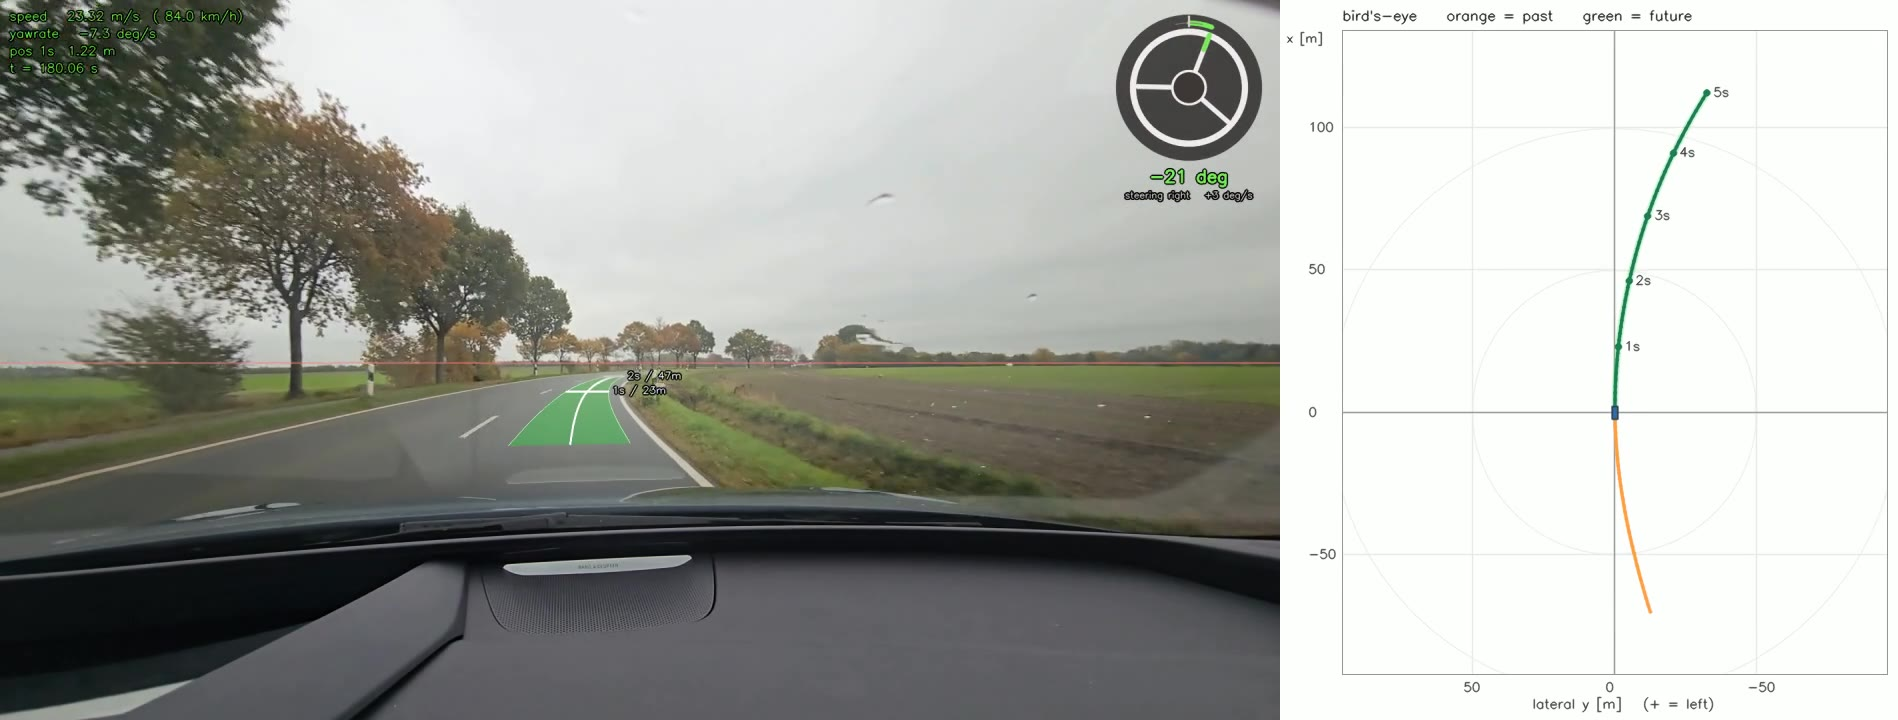
\includegraphics[width=\textwidth]{s24_overlay_30s.jpg}
\caption{S24 Ultra / A6 e-tron, $t = 180.06$\,s, 23.3\,m/s, yaw rate $-7.3^\circ$/s. The future path (green)
stays in the ego lane through the bend; the bird's-eye panel shows the same right turn that the GNSS bearing
confirms (118$^\circ \to$ 151$^\circ$ over 5\,s).}
\label{fig:s24}
\end{figure}

\begin{table}[H]
\centering\small
\begin{tabular}{@{}lc@{}}
\toprule
metric (\texttt{tools/verify\_overlay.py}, every 3rd frame) & value \\
\midrule
frames sampled / straight with both lines / curved or slow & 602 / 29 / 535 \\
path vs lane angle, median (p10, p90) & $-0.14^\circ$ ($-0.96^\circ$, $+0.84^\circ$) \\
offset from lane centre at 10\,m, median & $-0.06$ lane widths \\
offset from lane centre at 25\,m, median & $-0.05$ lane widths \\
ribbon centre inside the lane to 30\,m & 29 / 29 frames \\
ribbon edges (1.923\,m) inside the lane to 30\,m & 26 / 29 frames \\
prediction vs outcome at 20\,m, median (p10, p90) & $+0.01$\,m ($-0.87$, $+0.10$), $n=27$ \\
prediction vs outcome at 30\,m, median (p10, p90) & $+0.01$\,m ($-0.81$, $+0.14$), $n=24$ \\
\bottomrule
\end{tabular}
\caption{Corrected render, \meas{} (\texttt{verify\_fix.json}). The window is mostly bends, so only 29 frames
qualify as straight with two visible lines; the numbers are encouraging but a small sample, and the
$-0.8$\,m tail of prediction vs outcome is not yet explained. The full-length render and a check over all
11 minutes are the next step.}
\end{table}


%=====================================================================
\section{NVIDIA ViPE}
\label{sec:vipe}

ViPE (Huang et~al., ``ViPE: Video Pose Engine for 3D Geometric Perception'', NVIDIA, arXiv:2508.10934v1,
12 Aug 2025; code \url{https://github.com/nv-tlabs/vipe}) estimates camera intrinsics, poses and dense
near-metric depth from unconstrained video. The following is from the paper (\inh{}: not reproduced here).

\subsection{Pipeline (paper \S3.1)}
DROID-SLAM-style keyframe SLAM: (1) intrinsics initialised by GeoCalib on 4 sampled frames;
(2) keyframe selection when predicted motion (weighted dense flow plus sparse tracks) exceeds a threshold;
(3) frontend BA in a sliding window over recent keyframes, edges by temporal proximity or co-visibility,
Gauss--Newton; (4) backend BA over all keyframes with intrinsics unlocked, run at 8, 16, 64 keyframes and at
the end; (5) pose infilling of non-keyframes from their two nearest keyframes; (6) dense depth per frame.

\subsection{Formulation (paper Eqs.~1--5)}
Unknowns: poses $\{\mathbf{T}_i\in\mathrm{SE}(3)\}$, intrinsics $\bm k$, low-resolution keyframe depth
$\mathbf{D}_i\in\R^{H/8\times W/8}$:
\begin{equation}
e_\text{ViPE} = \sum_{(i,j)\in\mathcal E} e_\text{dense}(\mathbf T_i,\mathbf T_j,\mathbf D_i,\bm k)
+ \sum_{(i,j)\in\mathcal E} e_\text{sparse}(\mathbf T_i,\mathbf T_j,\mathbf D_i,\bm k)
+ \alpha\sum_{i\in\mathcal V} e_\text{depth}(\mathbf D_i),
\end{equation}
\begin{equation}
e_\text{dense} = \sum_{\bm u} w[\bm u]\,\big\|\Pi_{\bm k}\big(\mathbf T_j^{-1}\mathbf T_i\circ\Pi_{\bm k}^{-1}(\mathbf D_i[\bm u])\big) - \bm u - \mathbf F_{ij}[\bm u]\big\|^2,
\qquad
e_\text{depth} = \sum_{\bm u} m[\bm u]\,\big\|\mathbf D_i[\bm u] - \mathbf D_i^\text{prior}[\bm u]\big\|^2,
\end{equation}
where $\mathbf F_{ij}$ is the flow from a learned network (with the current geometry as a prior) and $w$ its
confidence; $e_\text{sparse}$ is the same reprojection for Shi--Tomasi corners tracked by Lucas--Kanade on the
full-resolution image (cuVSLAM), implemented by bilinear splatting into the flow form to keep the Hessian
structure; $\mathbf D^\text{prior}$ comes from a monocular metric depth network (Metric3Dv2 in all reported
experiments; UniDepthV2, UniK3D selectable) and is re-predicted when the intrinsics change. Solved by
Gauss--Newton with a factorised sparse solver and COLAMD ordering. \textbf{Dynamic masking}: GroundingDINO
boxes for user-specified classes prompt SAM at a fixed interval, propagated with XMem; the inverted mask
multiplies the flow weights and removes sparse tracks. \textbf{Camera models}: a radial model
$\bm u = (f q_{\bm k}(\theta)\cos\phi + W/2,\; f q_{\bm k}(\theta)\sin\phi + H/2)$ with principal point fixed at the
centre; pinhole $q = \tan\theta$; wide-angle by the unified camera model $q = \tan\theta/(1+\alpha\sqrt{\tan^2\theta+1})$,
$\bm k = [f, \alpha]$; rigs by $\mathbf T_v\mathbf T_i$; 360$^\circ$ as six cube-face pinholes.

\subsection{Dense depth alignment (paper Eq.~6)}
A video depth network gives affine-invariant $\mathbf D^\text{VDA}_i$; the BA geometry gives a sparse
$\mathbf D^\text{BA}_i$; per frame $\alpha_i,\beta_i = \arg\min \sum \|\mathbf M\cdot(\alpha/\mathbf D^\text{VDA} + \beta - 1/\mathbf D^\text{BA})\|^2$,
smoothed with momentum, $\mathbf D^\text{HD}_i = 1/(\hat\alpha_i/\mathbf D^\text{VDA}_i + \hat\beta_i)$; sparse coverage is
infilled with PriorDA.

\subsection{Reported results (\inh)}
TUM-RGBD: ATE 3.6\,cm (static), 1.5\,cm (dynamic), focal error 1.8$^\circ$/0.6$^\circ$, $\approx$3\,min per
$\approx$950 frames on an RTX 5090. KITTI (first 1024 frames, cropped to 512$\times$368): ATE 9.2\,m, focal error
1.9$^\circ$; RDS: ATE 5.0\,m, focal 7.9$^\circ$; 3--5\,FPS at 640$\times$480. Without ground truth they propose a
\emph{shuttle} metric (run the video forwards and reversed, compare) and the Sampson epipolar error. Ablation
(OpenDV): dense only S-ATE $1.39\cdot10^{-2}$; all terms with masking $1.05\cdot10^{-2}$. Datasets:
Dynpose-100K++ (99{,}501 videos, 15.7\,M frames), Wild-SDG-1M ($\approx$78\,M frames), Web360 ($\approx$2{,}000 videos);
$\approx$96\,M frames in total.

\subsection{Comparison}
\begin{table}[H]
\centering\small
\begin{tabularx}{\textwidth}{@{}lLL@{}}
\toprule
aspect & our pipeline & ViPE \\
\midrule
inputs & video + IMU + GNSS + orientation & video only \\
estimator & EKF forward + RTS backward over the session; 6 states & keyframe dense BA (Gauss--Newton) over poses, depth, intrinsics \\
metric scale & GNSS distance and speed; IMU & monocular metric-depth prior ($\alpha e_\text{depth}$) \\
time sync & explicit: PTS, coarse anchors, three-band gyro cross-correlation & not applicable \\
intrinsics & gyro regression, nominal FOV, plausibility gate; wrong on the ultra-wide & GeoCalib initialisation, refined in backend BA; unified model for wide lenses \\
camera motion & one mount per session (or an attitude track) & 6-DoF per frame \\
vehicle & phone$\to$vehicle frame, rear-axle reference, steering & none \\
road & ground plane, lanes, horizon & dense depth; no road model \\
dynamics & ignored & GroundingDINO + SAM + XMem masks \\
car interior & unhandled (S24 failure) & masked only if a class prompt matches \\
uncertainty & full covariance per instant; hold-out errors & BA residuals \\
self-checks & quality gates; prediction vs outcome & shuttle and Sampson metrics \\
compute & CPU; $\approx$0.4--0.75\,s per rendered 1080p frame & GPU; 3--5\,FPS \\
\bottomrule
\end{tabularx}
\end{table}

\noindent Our approach is strong where the vehicle and its sensors are known; ViPE where only pixels are. On
our recordings ViPE's learned intrinsics prior plus BA would have found the ultra-wide focal length, and
per-frame poses would have absorbed EIS motion without a hand-built track. It would not give a
vehicle-referenced trajectory or steering, its scale depends on how a depth network generalises to a
dashcam view, and nothing in it knows that a third of our frame is the inside of the car.

%=====================================================================
\section{Plan: a fused geometric video engine}
\label{sec:plan}

\subsection{Target formulation}
Replace the separate stages (sync, mount, EKF+RTS, calibration) by one sliding-window optimisation over
keyframes $i$ with states $\x_i$ (pose $\mathbf T_i\in\mathrm{SE}(3)$, velocity, IMU biases), the static
parameters $\Theta = \{\bm k, \mathbf R_{cv}, \bm t_v, \delta t\}$ (intrinsics with a distortion term,
camera-to-vehicle mount, sensor-to-video time offset) and low-resolution keyframe inverse depth $\mathbf D_i$:
\begin{equation}
\begin{aligned}
E = {}& \sum_i \|r_\text{IMU}(\x_i, \x_{i+1})\|^2_{\Sigma_\text{IMU}}
 + \sum_g \rho\big(\|r_\text{GNSS}(\x, t_g)\|^2_{\Sigma_g}\big)
 \\
 &+ \sum_{(i,j)} \sum_{\bm u\in\mathcal M_s} w_{ij}[\bm u]\,\big\|\Pi_{\bm k}\big(\mathbf T_{cj}^{-1}\mathbf T_{ci}\,\Pi_{\bm k}^{-1}(\bm u, \mathbf D_i[\bm u])\big) - \bm u - \mathbf F_{ij}[\bm u]\big\|^2 \\
 &+ \lambda_\text{road}\sum_i\sum_{\bm u\in\mathcal G_i} \big(\bm n^\top \mathbf X_i(\bm u) + h\big)^2
 + \lambda_\text{lane}\sum_i r_\text{lane}(\mathbf T_i, \Theta)^2 \\
 &+ \alpha\sum_i \|\mathbf D_i - s_i\,\mathbf D_i^\text{prior}\|^2_{m}
 + \|\Theta - \Theta_0\|^2_{\Sigma_\Theta},
\end{aligned}
\end{equation}
with IMU preintegration between keyframes, GNSS position/velocity/course factors with a robust loss $\rho$
(the Huber down-weighting of \S\ref{sec:ekf}), dense flow over the \emph{static} mask $\mathcal M_s$ (dynamic
objects \emph{and} car interior removed), a road-plane term on segmented ground pixels $\mathcal G_i$, lane
parallelism and width constancy, the depth prior with a free per-keyframe scale $s_i$ (so it cannot set
metric scale), and priors $\Theta_0$ from cheap measurements (gyro--image focal, lane VP). Camera poses are
$\mathbf T_{ci} = \mathbf T_i\,\mathbf T_{vc}(\Theta)$, so every image term constrains the vehicle trajectory
and the mount at once. The output is the smoothed vehicle trajectory with its marginal covariances, exactly
what \S\ref{sec:ekf} produces today, plus intrinsics, mount, time offset and depth.

\subsection{What is adopted from ViPE, and how it is developed further}
\begin{table}[H]
\centering\small
\begin{tabularx}{\textwidth}{@{}p{3.2cm}LL@{}}
\toprule
ViPE method & adopted as & developed further \\
\midrule
dense flow term $e_\text{dense}$ & image factor between keyframes & expressed through the \emph{vehicle} pose and mount; static mask includes the car interior, learned per recording from temporal variance and zero flow \\
sparse tracks $e_\text{sparse}$ & full-resolution corner tracks & dash and lane-marking ends as metric-scale anchors (the dash measurement that fixed $fh$ on the S24) \\
intrinsics in backend BA & $\bm k$ as a variable & initialised from gyro rotation vs far-field shift (which found the ultra-wide); plausibility set from the phone's real lens list \\
unified camera model & distortion parameter $\alpha$ & selected per lens; checked against straight lane lines \\
depth prior $\alpha e_\text{depth}$ & regulariser & free scale per keyframe, so GNSS/IMU set scale; prior--geometry disagreement logged as a domain-shift monitor \\
semantic masking & GroundingDINO/SAM-style masks & plus interior mask; plus ground segmentation for the road term \\
keyframes, frontend/backend & sliding window & IMU and GNSS factors marginalised at the window edge (bounded memory for hour-long drives) \\
shuttle metric & forward/reversed consistency & combined with our prediction-vs-outcome check and GNSS hold-out as release gates \\
\bottomrule
\end{tabularx}
\end{table}

\subsection{Work packages}
\begin{table}[H]
\centering\small
\begin{tabularx}{\textwidth}{@{}p{0.5cm}p{3cm}LL@{}}
\toprule
WP & package & content & pass criterion \\
\midrule
0 & Robust front end & resolution-independent thresholds; automatic interior/static mask; unified camera model & S24 recording calibrates with no override; mask IoU $\ge0.9$ \\
1 & Intrinsics from rotation & focal from far-field shift vs gyro, with distortion; lens-aware gate & $|f-f_\text{cb}| < 2\,\%$ vs checkerboard, main and ultra-wide \\
2 & Fused optimiser & IMU preintegration + GNSS + dense flow; $\Theta$ including time offset; replaces EKF+RTS and mount calibration & hold-out position RMS $\le$ today; prediction-vs-outcome at 30\,m $\le0.2$\,m median \\
3 & Road and lane factors & ground-plane and lane terms; separates $f$ from $h$ with GNSS scale & $h$ within 3\,cm of tape; $v_h$ within 3\,px of lane-width estimate \\
4 & Time-varying mount & spline rotation for EIS / loose holders, from car-fixed features and image--gyro residuals & EIS recording: path-vs-lane within $\pm0.5^\circ$ in every 5\,s bin \\
5 & Depth prior as regulariser & scale-free prior; ablation & GNSS scale unchanged when the prior is dropped \\
6 & Dynamics and long drives & masks for vehicles and people; marginalising window; loop closure & no degradation in dense traffic; constant memory at 1\,h \\
7 & Evaluation harness & per recording: trajectory hold-out, intrinsics vs checkerboard, mount vs tape, drawing error per time bin; plus KITTI/nuScenes & runs on every release; regressions fail CI \\
\bottomrule
\end{tabularx}
\end{table}

\paragraph{Order.} WP0 and WP1 first (days; they make the S24 recording work without manual overrides) with
WP7 in parallel; then WP2 with WP3 (weeks); WP4--6 after. Code and models are chosen independently of ViPE
and their licences checked (ViPE is Apache-2.0 with non-commercial components).

%=====================================================================
\section{Recording recommendations}
\begin{itemize}
\item Record with the main (1$\times$) camera at 1080p unless the ultra-wide is wanted; note the lens. Keep
  stabilisation off.
\item Mount rigidly, with as little dashboard in view as possible.
\item Measure camera height and lateral position once per mount; one checkerboard video per phone and lens.
\item Start with ten seconds stationary (gyro bias, gravity reference).
\end{itemize}

\section{Limitations}
\begin{itemize}
\item The S24 corrected calibration is measured on one 60\,s window and assumes a distortion-corrected
  ultra-wide image; it is not yet validated over the full 11 minutes.
\item ViPE results are \inh{} from the paper; several AUDIT.md figures are \inh{} from the original project.
\end{itemize}

\end{document}
